\subsection{Summary of Completed Research}

To measure the reputation of authors, the system analyzes
the revision history of all wiki articles, in
chronological order.
The evolution of an article is tracked using a granularity
of words (as opposed to characters or sentences),
with an author being assigned to each word.
Suppose that an author \editor{k} contributes to a Wikipedia article by
performing an edit $\revision{k}: \version{k-1} \goesto \version{k}$
from version \version{k-1} to
version \version{k}.
When another author \editor{j} subsequently performs an edit
$\revision{j}: \version{j-1} \goesto \version{j}$
of the same article ($j > k$), author \editor{j}
implicitly gives a judgment on the quality of \editor{k}'s contribution, by
preserving it or removing it.
The reputation system relies on these judgments, in two forms, to increase
or decrease the reputation of \editor{k}: \textit{text survival}
and \textit{edit survival}~\cite{www07}.

\subsubsection*{Text Survival}

\begin{figure}[t]
\centering
\subfigure[Graphical representation of the \textit{text survival} over
    several subsequent revisions.]{
\label{fig-textcontr-a} 
\framebox{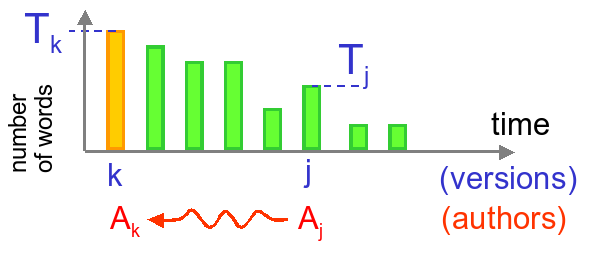
\includegraphics[width=0.42\textwidth]{part-F20-rep/textcontr-2}}
}
\hspace{1ex}
\subfigure[Calculating the \textit{text longevity} of a contribution.]{
\label{fig-textcontr-b}
\framebox{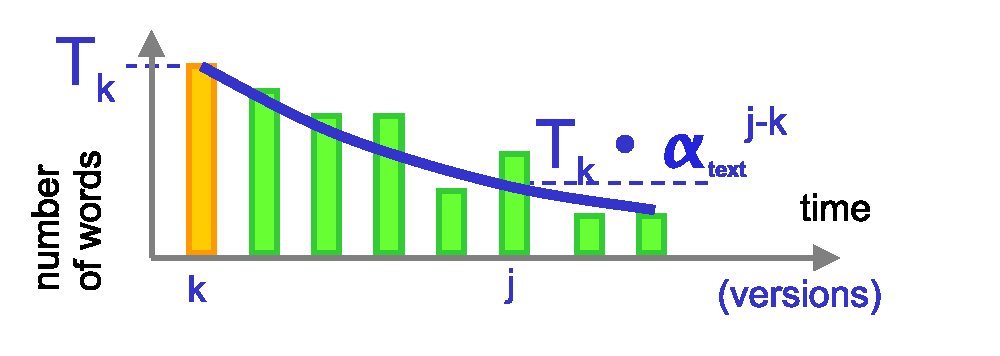
\includegraphics[width=0.48\textwidth]{part-F20-rep/text-longevity}}
}
\caption{A graphical depiction of how a text contribution survives
	through future revisions.
	An author, \editor{k}, adds $T_k$ words in version \version{k}.
	In subsequent versions, only a portion of the words survive.
	We model the survival over time as a geometric curve,
	to arrive at a single number describing the longevity
	of the initial contribution.}
\label{fig-textsurvival}
\end{figure}


  The basic idea of text survival is to track the text introduced in
  \version{k}, and measure how many of those words are
  still present in \version{j}.
  Referring to Figure~\ref{fig-textcontr-a}, the judgement
  that author \editor{j} makes is the
  decision to preserve $T_j / T_k$ of the words introducted
  by \editor{k} in \version{k}, where
  $T_j = \txt(j,j)$ and $T_k = \txt(k,k)$.
  When the edit \revision{j} occurs, if
  $k < j \leq k+10$ and $\editor{k} \neq \editor{j}$,
  we add to the reputation
  of \editor{k} the amount:
  \[
    \coeffrep \cdot \coefftext \cdot \frac{T_j}{T_k}
    \cdot (T_k)^\lengthexp \cdot \log(1 + \rep(\editor{j},\revision{j}))
  \]
  where $\coeffrep > 0$, $\coefftext \in [0,1]$, and $\lengthexp \in
  [0,1]$ are parameters, and where $\rep(\editor{j},\revision{j})$
  is the reputation of \editor{j} at the time \revision{j} is performed.

  To measure the overall quality of a single text contribution
  (see Figure~\ref{fig-textcontr-b}), we model the sequence of
  words preserved over time as a geometric curve; we call the
  value which describes the curve
  the text longevity, \tlong, of a text contribution at \revision{k}.
  Specifically, we solve the following equation for $\tlong(\revision{k})$:
  \begin{equation*}
  	\sum_{i=k+1}^n T_i = T_k \cdot
		\sum_{i=k}^n \{ \tlong(\revision{k}) \}^{i-k}
  \end{equation*}
  This value ranges from zero for a contribution which is immediately
  reverted, to one for a text contribution which is never modified.
  The intuition behind a geometric model is that if an edit is
  ``bad,'' then most of the text will be removed right away.
  As time passes, the size of the edits gets smaller and
  the text tends to stabilize into a form
  that people can agree on, until it eventually no longer changes.

  In order to set the parameters for our reputation function,
  we wrote a search function to optimize for the highest
  correlation between the reputation of an author (which is
  based on past contributions at the time of edit \revision{k})
  and the text longevity of the contribution of \revision{k}
  (which is based on information from future edits).

\subsubsection*{Edit Survival}

\begin{figure}[t]
\centering
\subfigure[Graphical representation of a good edit contribution.]{
\label{fig-editcontr-a} 
\framebox{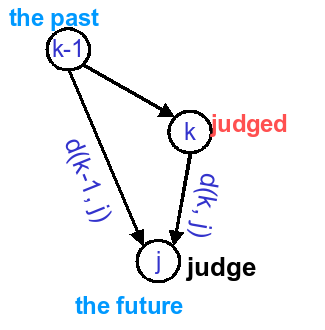
\includegraphics[width=0.35\textwidth]{part-F20-rep/editcontr-good}}
}
\hspace{1ex}
\subfigure[Graphical representation of a bad edit contribution.]{
\label{fig-editcontr-b}
\framebox{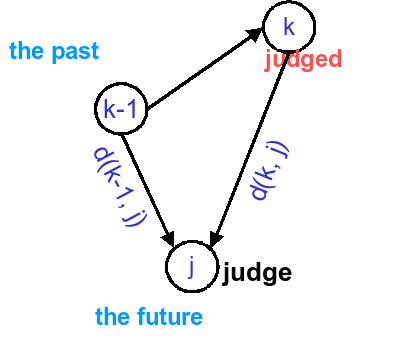
\includegraphics[width=0.40\textwidth]{part-F20-rep/editcontr-bad}}
}
\caption{To measure the quality of version \version{k}, we also
	look at the previous version \version{k-1} and some future
	version \version{j}.
	The three versions form a triangle, using
	edit distance~\cite{Levenshtein66} to define the separation
	between each other.
	Intuitively, we know that when \version{k} is good,
	the distance to the future, $\dist(\version{k},\version{j})$,
	will be shorter than if \version{k} is bad.
	(When \version{k} is bad, more editing is required to
	bring it back to a better version, plus the editing
	to bring it to the future.)
}
\label{fig-editcontr}
\end{figure}

\hyphenation{re-arrang-ed}
  We would like to have a similar notion of survival for edits,
  particularly for the case where text is rearranged by an author
  different from the author who introduced the text.
  To accomplish this, we utilize the
  \intro{edit distance}~\cite{Levenshtein66,TichyEditDist,EditDistanceMoves,www07}
  --- a measure of how many word insertions, deletions,
  and transpositions are needed to change one revision into the other ---
  to measure how different one version is from another.
  To turn this into a quality metric for the
  version \version{k}, we look at edits done as part of \revision{k}
  and ask ``does the work done bring us closer to how the page
  will look in the future?''
  If future versions incorporate and build on the changes of edit \revision{k},
  then the edits are of good quality.
  When future versions mostly undo or discard the work of \revision{k},
  then the edits are of bad quality.

%\begin{wrapfigure}{r}{0.55\textwidth}
\begin{figure}
\centering
\framebox{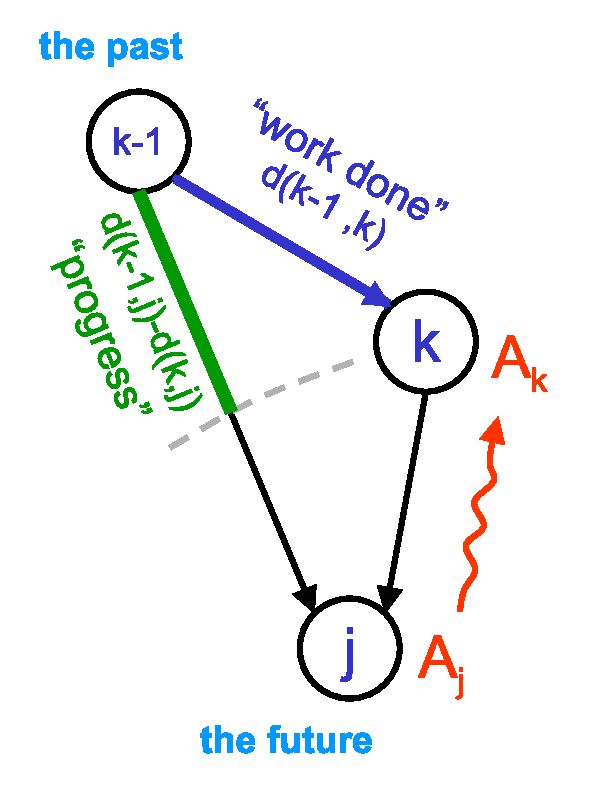
\includegraphics[width=0.35\textwidth]{part-F20-rep/edit-longevity}}
\caption{Quality is measured by calculating how much \textit{progress}
	is made towards the future version of the article,
	and dividing that by the amount of \textit{work done}
	during the edit.}
\label{fig-editlong}
\end{figure}
%\end{wrapfigure}


  To calculate the quality of an edit \revision{k},
  we additionally consider two \intro{reference versions}:
  the immediate past \version{k-1} and some future version \version{j}.
  These three points allow us to define a triangle
  (see the two examples in Figure~\ref{fig-editcontr})
  using the edit distances $d(\version{k-1},\version{k})$,
  $d(\version{k-1},\version{j})$ and $d(\version{k},\version{j})$.
  We then computes the ratio
  \begin{equation*}
  \editq(\version{k},\version{j}) = \bigl[ \dist(\version{k-1},\version{j})
  		- \dist(\version{k},\version{j}) \bigr]
	/ \dist(\version{k-1},\version{k})
  \end{equation*}
  between the ``useful work''
  $\dist(\version{k-1},\version{j}) - \dist(\version{k},\version{j})$ and the
  ``total work'' $\dist(\version{k-1},\version{k})$
  (see Figure~\ref{fig-editlong} for a pictorial representation).
  The ``total work'' $\dist(\version{k-1},\version{k})$
  is a measure of how much change
  was performed during the
  edit $\revision{k}: \version{k-1} \goesto \version{k}$;
  the ``useful work''
  $\dist(\version{k-1},\version{j}) - \dist(\version{k},\version{j})$
  is a measure of
  how much closer the article becomes to the future version \version{j}.
  For reverted edits, the ratio $\editq(\version{k},\version{j})$
  is $-1$, since all of the work
  goes into \textit{increasing} the distance between \version{k} and \version{j}.
  For edits that are preserved, $\editq(\version{k},\version{j})$ is close to~1.
  The \intro{edit longevity}, \elong, of edit \revision{k} is then taken to
  be the average edit quality as judged by the next three revisions:
  \begin{equation*}
      \elong(\revision{k}) = \sum_{i=k+1}^{\min(k+3, n)}
      		\editq(\version{k},\version{i})
  \end{equation*}

  Updating the reputation of author \editor{k} for their editing
  work is based on this notion of edit longevity.
  When edit \revision{j} occurs, if
  $k < j \le k+3$ and $\editor{k} \ne \editor{j}$,
  we first compute the value:
  \begin{equation*}
  	q := \frac{ \slack \cdot \dist(\version{k-1},\version{j})
		- \dist(\version{k},\version{j}) }
		{ \dist(\version{k-1},\version{k}) }
  \end{equation*}
  If $q < 0$, we update this value to include a punishment factor,
  $q := q \cdot \coeffpunish$.
  The reputation for \editor{k} is then updated according to:
  \begin{equation*}
  	q \cdot \coeffrep \cdot (1 - \coefftext) \cdot
	        (\dist(\version{k-1},\version{k}))^\lengthexp
		\cdot \log(1 + \rep(\editor{j},\revision{j}))
  \end{equation*}
  where $\coeffpunish \geq 1$, $\slack \geq 1$, $\coeffrep > 0$,
  $\coefftext \in [0,1]$, and $\lengthexp \in [0,1]$ are parameters,
  and $\rep(\editor{j},\revision{j})$ is the reputation
  of~$\editor{j}$ at the time~$\revision{j}$ is performed.
  As with the text survival parameters, we used a search function
  to discover optimal parameter values, so that there was a high
  correlation between author reputation and the edit longevity
  of edit \revision{k}.


\subsubsection*{Quantitative Evaluation}

\begin{table}
\begin{center}
\begin{tabular}{|r|c|c|} \hline
Longevity & Judged bad & Judged good \\ \hline
\multicolumn{1}{|l|}{Short-lived edits: \qquad \quad} & & \\[1ex]
   Low [0.0--0.2]   &    66  \% &    19 \% \\
Normal [0.2--1.0]   &    16  \% &    68 \% \\ \hline
\multicolumn{1}{|l|}{Short-lived text: \qquad \quad} & & \\[1ex]
   Low [0.0--0.2]   &    74  \% &    13 \% \\
Normal [0.2--1.0]   &    14  \% &    85 \% \\ \hline
\end{tabular}
\end{center}
\caption{User ratings of short-lived edits and text from the
  Italian Wikipedia, as a function of author reputation.
  We presented edit differences to a test group of users;
  we selected edits that had
  low text longevity or low edit longevity,
  and asked users to rate whether the edit was good or bad.
  In square brackets, we give the
  interval where the normalized value $\log(1+r) / \log (1 +
  \coeffmaxrep)$ of a reputation $r$ falls.  The precentages do not
  add to 100\%, because users could also rank a change as ``neutral''.}
\label{tbl:human}
\end{table}

\begin{table}
\begin{center}
\begin{tabular}{|l||c|c||c|c|} \hline
 & \multicolumn{2}{|c||}{Precision}
 & \multicolumn{2}{|c|}{Recall} \\
 & Edit & Text & Edit & Text \\[0.5ex] \hline
{\bf Italian Wikipedia:} & & & &    \\
\qquad Content-driven reputation & 14.15 &  3.94 & 19.39 & 38.69 \\
\qquad Edit count as reputation  & 11.50 &  3.32 & 19.09 & 39.52 \\ \hline
{\bf French Wikipedia:} & & & & \\
\qquad Content-driven reputation & 23.92 &  5.85 & 32.24 & 37.80 \\
\qquad Edit count as reputation &  21.62 &  5.63 & 28.30 & 37.92 \\ \hline
\end{tabular}
\end{center}
\caption{Summary of the performance of content-driven reputation over
the Italian and French Wikipedias. All data are expressed as percentages.
Precision is the probability that the text or edit longevity is low,
given that the reputation is low.
Recall is the probability that the reputation is low, given that
the text or edit longevity is low.
}
\label{tbl:comparison-with-count}
\end{table}



We have evaluated the effectiveness of the
reputation system in two ways.
The first evaluation involved the human judgements of seven volunteers on
680 edits from the Italian Wikipedia;
each participant could rate
an edit as ``good,'' ``bad'' or ``neutral.''
We averaged the judgements of the participants, and
compared these results to the predictions made
by the reputation of the authors of the edits.
The results, presented in Table~\ref{tbl:human},
show that low reputation is a very good predictor
of bad short-lived text.
Using these results, we computed the approximate
recall factors on the Italian Wikipedia; what fraction
of the changes judged \textit{bad} by humans did our
content-driven reputation system identify by assigning low-reputation
to the author:
\begin{itemize}
\item The recall for short-lived edits that are judged to
    be bad is over 49\%.
\item The recall for short-lived text that is judged to
    be bad is over 79\%.
\end{itemize}

Our second evaluation was to measure the \textit{predictive}
power of our reputation system, and compare it to the
\textit{edit-count} reputation system.
It is commonly believed that, as Wikipedia authors gain
experience (through revision comments, talk pages,
and reading articles on Wikipedia standards), the quality
of their submissions goes up.
Hence, it is reasonable to take edit count --- the number of edits
performed by the author --- as a form of reputation.

We considered edits to the Italian and French Wikipedias, and
for each revision, we noted the reputation of the author at the
moment the change was made (which is based on past changes by the author),
and we computed the text and edit longevity of the change (which
is based on future edits to the same article).
Some results are presented in Table~\ref{tbl:comparison-with-count};
other metrics are additionally presented in~\cite{www07}.
We believe that one reason the edit-count based reputation
performs well in our measurements is that authors, after
performing edits that are criticized and reverted,
commonly either replace their identity or stop contributing altogether.
The edit-count reputation system could never work in the live Wikipedia, however,
as authors would change their behavior to maximize their edit count.

